\documentclass[a4paper]{article}
\usepackage[T1]{fontenc}
\usepackage{minted}
\usepackage{bera}

\usepackage{amssymb,amsmath,amsthm,amsfonts}
\usepackage{mathtools}
\usepackage{multicol,multirow}
\usepackage{calc}
\usepackage{enumerate,float,graphics,graphicx}
\usepackage{ifthen}
\usepackage{setspace}
\usepackage[dvipsnames]{xcolor}
\usepackage{subfig}
\usepackage{geometry}

\usepackage{listings}

\ifthenelse{\lengthtest { \paperwidth = 11in}}
    { \geometry{top=.5in,left=.5in,right=.5in,bottom=.5in} }
	{\ifthenelse{ \lengthtest{ \paperwidth = 297mm}}
		{\geometry{top=1cm,left=1cm,right=1cm,bottom=1cm} }
		{\geometry{top=1cm,left=1cm,right=1cm,bottom=1cm} }
	}

\pagestyle{empty}
\makeatletter
\renewcommand{\section}{\@startsection{section}{1}{0mm}%
                                {-1ex plus -.5ex minus -.2ex}%
                                {0.5ex plus .2ex}%x
                                {\normalfont\large\bfseries}}
\renewcommand{\subsection}{\@startsection{subsection}{2}{0mm}%
                                {-1explus -.5ex minus -.2ex}%
                                {0.5ex plus .2ex}%
                                {\normalfont\normalsize\bfseries}}
\renewcommand{\subsubsection}{\@startsection{subsubsection}{3}{0mm}%
                                {-1ex plus -.5ex minus -.2ex}%
                                {1ex plus .2ex}%
                                {\normalfont\small\bfseries}}
\makeatother
%\setcounter{secnumdepth}{0}
\setlength{\parindent}{0pt}
\setlength{\parskip}{0pt plus 0.5ex}



\usepackage{xcolor}

\definecolor{codegreen}{rgb}{0,0.6,0}
\definecolor{codegray}{rgb}{0.5,0.5,0.5}
\definecolor{codepurple}{rgb}{0.58,0,0.82}
\definecolor{backcolour}{rgb}{0.95,0.95,0.92}

\lstdefinestyle{mystyle}{
    backgroundcolor=\color{backcolour},   
    commentstyle=\color{codegreen},
    keywordstyle=\color{magenta},
    numberstyle=\tiny\color{codegray},
    stringstyle=\color{codepurple},
    basicstyle=\ttfamily\footnotesize,
    breakatwhitespace=false,         
    breaklines=true,                 
    captionpos=b,                    
    keepspaces=true,                 
%    numbers=left,                    
    numbersep=5pt,                  
    showspaces=false,                
    showstringspaces=false,
    showtabs=false,                  
    tabsize=2
}

\lstset{style=mystyle}









\usepackage[colorlinks=true,citecolor=blue,linkcolor=blue]{hyperref}



% -----------------------------------------------------------------------

\title{}
%\doublespacing
\begin{document}

\raggedright
\footnotesize

\begin{center}
     \Large{\textbf{EEC 242 - VHDL cheat sheet\footnote{ \textcolor{darkgray}{Taha Ahmed}}}} \\
    \textbf{Chapter 1 and 2}
\end{center}
%\begin{multicols}{2}
%\setlength{\premulticols}{1pt}
%\setlength{\postmulticols}{1pt}
%\setlength{\multicolsep}{1pt}
%\setlength{\columnsep}{2pt}


\section{Chapter 1}

\begin{itemize}
\item VHDL $\Rightarrow$ \textbf{V}ery High Speed Integrated Circuits \textbf{H}ardware \textbf{D}escription \textbf{L}anguage

\item VHDL is a concurrent language.

\item VHDL is not case sensitive.

\item Purpose:
\begin{itemize}
\item Documentation
\item Simulation
\end{itemize}

\item Documentation : write a comment\\
Characters "\texttt{- -}"

\subsection{Entity}
\item Entity deceleration defines the name of the entity and lists the input and output ports.

\begin{minted}{vhdl}
entity example1 is 
   port(x1, x2, x3     :in    std_logic;
        in1            :in    integer;
        val1           :out   std_logic;
        val2           :out   std_logic_vector(3 downto 0));
end example1;
\end{minted}

\subsubsection{Signals Names}

\item Signal Name specifies external interface signals
\item It can be any alphanumeric character
\item Rules:
\begin{itemize}
\item Must begin with a letter (Don't begin with number or \_)
\item Don't end with underscore \_
\item No two successive underscores \_ \_
\end{itemize}

\subsubsection{Modes}

\item Indicate signal direction:
%\begin{itemize}
%\item in : input
%\item out : output (whose value can only be read by other entities)
%\item buffer : output (whose value can be read inside the entity's architecture)
%\item inout :  can be an input or an output.
%\end{itemize}

\begin{tabbing}
\hspace{1.1cm}\=\hspace{1.3cm}\=\kill
- in  \> : input \>   \\ 
- out  \> : output \> (whose value can only be read by other entities) \\ 
- buffer  \> : output \> (whose value can be read inside the entity's architecture) \\ 
- inout  \>  : can be an input or an output. \>  
\end{tabbing} 



\subsubsection{Types}

\item A built in or user defined signal type:
%\begin{itemize}
%\item in : input
%\item out : output (whose value can only be read by other entities)
%\item buffer : output (whose value can be read inside the entity's architecture)
%\item inout :  can be an input or an output.
%\end{itemize}

\begin{tabbing}
\hspace{2.4cm}\=\hspace{1.3cm}\=\kill
- bit  \> : 0 or 1. \>   \\ 
- bit\_vector  \> : vector of bits. \>  \\ 
- std\_logic  \> : 0, 1, Z, -, L, H, U, X, W. \>  \\ 
- std\_logic\_vector  \>  : vector of std\_logics. \>   \\
- boolean  \> : TRUE or FALSE. \>   \\ 
- integer  \> : integer numbers. \>   \\ 
- real  \> : real numbers. \>   \\ 
- character  \> : character. \>   \\ 
- time  \> : time. \>   \\ 


\end{tabbing} 


\item bit \& bit\_vector :
\begin{itemize}
\item bit : 0 or 1.

\item
\begin{minted}{vhdl}
port (C    : in bit;
      BYTE : in bit);
\end{minted}
\item bit\_vector : multi-bit data



\item Diffrence between \texttt{to} and \texttt{downto}
\begin{minted}{vhdl}
port (to_example     : out bit-vector(1 to 8);
      downto_example : out bit-vector(7 downto 0));
\end{minted}

\item \texttt{to\_example <= "10011000"} results in \\ \texttt{to\_example(1) = 1}\\
\texttt{to\_example(2) = 0}\\
\texttt{to\_example(3) = 0}\\
\texttt{to\_example(4) = 1}\\
\texttt{to\_example(5) = 1}\\
\texttt{to\_example(6) = 0}\\
\texttt{to\_example(7) = 0}\\
\texttt{to\_example(8) = 0}\\

\item \texttt{downto\_example <= "10011000"} results in \\ \texttt{downto\_example(7) = 1}\\
\texttt{downto\_example(6) = 0}\\
\texttt{downto\_example(5) = 0}\\
\texttt{downto\_example(4) = 1}\\
\texttt{downto\_example(3) = 1}\\
\texttt{downto\_example(2) = 0}\\
\texttt{downto\_example(1) = 0}\\
\texttt{downto\_example(0) = 0}\\





\end{itemize}
\item std\_logic \& std\_logic\_vector.
\begin{itemize}
\item to use this type
\begin{minted}{vhdl}
Library IEEE;
Use IEEE.std_logic_1164.all;
\end{minted}

\item \texttt{
1 \\
0 \\
Z: high impedance \\
-: don't care\\
U: uninitialized\\
X: unknown\\
W: weak unknown\\
L: weak high\\
H: weak low}

\end{itemize}

\item Integer:
\begin{itemize}
\item represents a binary number

\item by default, it has 32 bits, range from $-(2^{31}-1)$ to $2^{31}-1$.
\item you can declare integer with fewer bits by  \texttt{Range} keyword :
\begin{minted}{vhdl}
Integer Range -127 to 127;
\end{minted}
\end{itemize}

\item Generic:
\begin{itemize}
\item \begin{minted}{vhdl}
entity example1 is 
   Generic (Delay : Time := 10ns);
   port(x1, x2, x3   :in    std_logic;
        in1          :in    std_logic;
        in2          :in    std_logic;
        output       :out   std_logic;
        val2         :out   std_logic_vector(3 downto 0))
end example1;
Architecture Behavior of example1 is
begin
...
 output  <=  in1 or in2 after Delay;
...
end Behavior;
\end{minted}
---------------------
\begin{minted}{vhdl}
entity CPU is 
   Generic (BusWidth : Integer := 16);
   port(DataBus : inout std_logic_vector (BusWidth downto 0));
end Cpu;

\end{minted}


\end{itemize}


\subsection{Architecture}
\item  specifies how the circuit operates and how it is implemented.
\item Ways
\begin{itemize}
\item Behavioral (Data flow / Sequential)
\item Structural
\item Combination of both
\end{itemize}

\subsubsection{Operators}
\item From Highest Precedence to Lowest:\\
\texttt{** : exponentiation\\
ABS\\
Not\\
*\\
/\\
MOD\\
REM\\
+\\
-\\
\&  : Concatenation\\
=\\
/= : Not equal\\
<\\
<=\\
>\\
>=\\
AND\\
OR\\
NAND\\
NOR\\
XOR\\
XNOR\\
NOT\\}

\begin{minted}{vhdl}
entity example1 is 
   port(x1, x2, x3   :in    std_logic;
        output       :out   std_logic);
end example1;

Architecture Behavior of example1 is
begin

 output  <=  (x1 and x2) or ( not x2 and x3);

end Behavior;
\end{minted}

\subsubsection{Signals}
\item Represents logic signals or wires in a circuit.
\item Signals assignment operator \texttt{<=}
\item \texttt{Signal signal\_name : type;} 
\item 
\begin{minted}{vhdl}
entity example1 is 
   port(x1, x2, x3   :in    std_logic;
        output       :out   std_logic);
end example1;

Architecture Behavior of example1 is
Signal A, B : std_logic;
begin

A <= x1 and x2;
B <= not x2 and x3;
output  <=  A or B;

end Behavior;
\end{minted}

\subsection{Concurrent Assignment Statements}
\item to \textbf{assign a value to a signal} in an architecture body.
\item Four types:
\begin{itemize}
\item Simple signal assignment.
\item Selected signal assignment.
\item Conditional signal assignment.
\item Generate statements.
\end{itemize}

\subsubsection{Simple Signal Assignment}
\item For a logic or arithmetic expression.
\begin{minted}{vhdl}
output  <=  (x1 and x2) or ( not x2 and x3);
\end{minted}

\item Assign using Others:\\
Instead of writing \texttt{S <= "00000000";}\\
write \texttt{S <= (others => '0');}

\subsubsection{Selected Signal Assignment}
\item Assign the value of a signal to a \textbf{one of several alternatives based on a selection} criterion
\begin{minted}{vhdl}
WITH some_selector SELECT
    	output <= x1 WHEN '0',
    	          x2 WHEN OTHERS;
\end{minted}

\subsubsection{Conditional Signal Assignment}
\item Assign the value of a signal to a \textbf{one of several alternatives based on a Condition} 
\begin{minted}{vhdl}
    output <= '1' WHEN x1 = x2 ELSE
    	      '0';
\end{minted}

\begin{minted}{vhdl}
-- Priority Circuit

-- Libraries to use std_logic
Library IEEE;
Use IEEE.std_logic_1164.all;

-- Entity
Entity priority is 
   port(x1, x2, x3   :in    std_logic;
        output       :out   std_logic_vector (1 downto 0));
end priority;

-- Architecture
Architecture Behavior of priority is

begin

output  <=  "01" when x1 = '1' else
            "10" when x2 = '1' else
            "11" when x3 = '1' else
            "00" ;


end Behavior;

\end{minted}

\subsubsection{Generate Signal Assignment}
\item types
\begin{itemize}
\item \texttt{for} generate.
\item \texttt{if} generate.
\end{itemize}


\begin{minted}{vhdl}

-- Libraries to use std_logic
Library IEEE;
Use IEEE.std_logic_1164.all;

-- Entity
Entity example is 
   port(input_signal     :in    std_logic_vector (15 downto 0);
        first_output     :out   std_logic_vector (7 downto 0);
        second_output    :out   std_logic_vector (0 to 7));
end example;

-- Architecture
Architecture Behavior of example is

begin

GENERATE_EXAMPLE : for i in 0 to 7 generate
                       first_output(i) <= input_signal(i);
                       second_output(7 - i) <= input_signal(i + 8);

end generate GENERATE_EXAMPLE;

end Behavior;

-- take a moment and try to understand this code.
-- the code breaks the input to two halves, assign 
-- the first half to the first out and
-- the reverse of the second halve to the second out
-- input = "1110101100010110"
-- first_output = "00010110"
-- second_output = "11010111"
\end{minted}

\section{Chapter 2}
\subsection{Components}|

\item Intro:\\
VHDL entity defined in one file can be used as a subcircuit in another file.
\item The subcircuit is called a component.
\item Where is the deceleration?\\
 in the declaration region of an architecture.

\item Example: Full adder
\begin{minted}{vhdl}

-- Libraries to use std_logic
Library IEEE;
Use IEEE.std_logic_1164.all;

-- Entity
Entity fullAdder1bit is 
   port(x, y, carryIn     :in    std_logic;
        sum, carryOut     :out   std_logic);
end fullAdder1bit;

-- Architecture
Architecture Behavior of example is

begin

sum <= x xor y xor carryIn;
carryOut <= (x and y) or (x and carryIn) or (y and carryIn);

end Behavior;

\end{minted}

\item Example: 4 bit Full adder
\begin{minted}{vhdl}

-- Libraries to use std_logic
Library IEEE;
Use IEEE.std_logic_1164.all;

-- Entity
Entity fullAdder4bit is 
   port(x, y     :in    std_logic_vector(3 downto 0);
        carryIn  :in    std_logic;
        sum      :out   std_logic_vector(3 downto 0);
        carryOut :out   std_logic);
end fullAdder4bit;

-- Architecture
Architecture Behavior of example is

-- Here we declare an intermediate signal to help us to contain carry of each stage

Signal helpMe :  std_logic_vector(1 to 3);

-- Here we declare a component, our 1 bit full adder

Component fullAdder1bit
   port(x, y, carryIn     :in    std_logic;
        sum, carryOut     :out   std_logic);
end Component;

begin

stage0 : fullAdder1bit PORT MAP (carryIn, x(0), y(0), sum(0), helpMe(1));
stage1 : fullAdder1bit PORT MAP (helpMe(1), x(1), y(1), sum(1), helpMe(2));
stage2 : fullAdder1bit PORT MAP (helpMe(2), x(2), y(2), sum(2), helpMe(3));
stage3 : fullAdder1bit PORT MAP (helpMe(3), x(3), y(3), sum(3), carryOut);

-- YOU CAN ALSO TYPE
-- stage3 : fullAdder1bit PORT MAP (x => x(3), y => y(3),
--                        carryIn => helpMe(3), sum => sum(3), carryOut => carryOut);

end Behavior;

\end{minted}


\item Example: 4 bit Full adder (another implementation using for generate)
\begin{minted}{vhdl}

-- Libraries to use std_logic
Library IEEE;
Use IEEE.std_logic_1164.all;

-- Entity
Entity fullAdder4bit is 
   port(x, y     :in    std_logic_vector(3 downto 0);
        carryIn  :in    std_logic;
        sum      :out   std_logic_vector(3 downto 0);
        carryOut :out   std_logic);
end fullAdder4bit;

-- Architecture
Architecture Structure of example is

-- Here we declare an intermediate signal to help us to contain carry of each stage

Signal helpMe :  std_logic_vector(0 to 4)


Component fullAdder1bit
   port(x, y, carryIn     :in    std_logic;
        sum, carryOut     :out   std_logic);
end Component;


begin

helpMe(0) <= CarryIn;

GENERATE_LABEL : for i in 0 to 3 generate
                    fullAdder1bit PORT MAP (helpMe(i), x(i), y(i), sum(i), helpMe(i + 1)); 
               
end generate GENERATE_LABEL;     
carryOut <= helpMe(4);
end Structure;

\end{minted}


\item Example: 4 bit Full adder (another implementation)
\begin{minted}{vhdl}


Library IEEE;
Use IEEE.std_logic_1164.all;
Use IEEE.std_logic_signed.all;

Entity fullAdder4bit is 
   port(x, y     :in    std_logic_vector(3 downto 0);
        carryIn  :in    std_logic;
        sum      :out   std_logic_vector(3 downto 0);
        carryOut :out   std_logic);
end fullAdder4bit;


Architecture Behavior of example is

-- Here we declare an intermediate signal to help us, it will be the summation of x, y and carryIn, then we will break it to sum and carry

Signal helpMeSum :  std_logic_vector(4 downto 0);

-- No need to components here!

begin

helpMeSum <= ('0' & x) + y + carryIn;
sum <= helpMeSum(3 downto 0);
carryOut <= helpMeSum(4);

end Behavior;

\end{minted}


\item Example: Multiplexers 4to1
\begin{minted}{vhdl}

-- Libraries to use std_logic
Library IEEE;
Use IEEE.std_logic_1164.all;

-- Entity
Entity mux4to1 is 
   port(w0,w1,w2,w3     :in    std_logic;
        selector        :in    std_logic_vector(1 downto 0);
        output          :out   std_logic);
end mux4to1;

-- Architecture
Architecture Behavior of mux4to1 is

begin 

With selector select 
	output <= w0 when "00",
              w1 when "01",
              w2 when "10",
              w3 when others;
end Behavior;

\end{minted}

\item Example: Multiplexers 16to1 using 4to1 mux

\begin{figure}[H] 
	\centering
	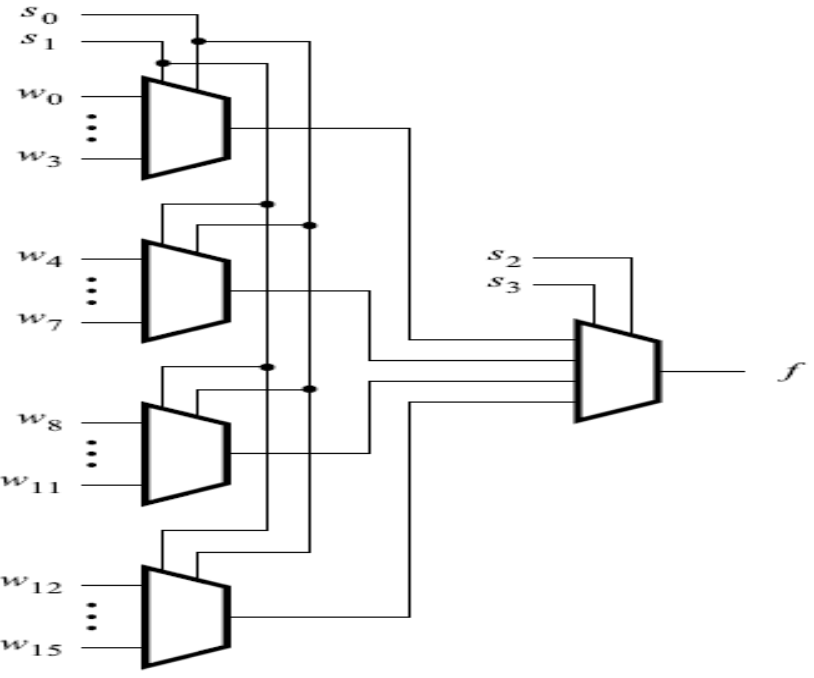
\includegraphics[width=0.5\textwidth]{Multiplexers 16to1 using 4to1 mux}
%	\caption{}
	\label{fig:raw data}
\end{figure}


\begin{minted}{vhdl}

-- Libraries to use std_logic
Library IEEE;
Use IEEE.std_logic_1164.all;

-- Entity
Entity mux16to1 is 
   port(w           :in    std_logic_vector (0 to 15);
        selector    :in    std_logic_vector(3 downto 0);
        output      :out   std_logic);
end mux16to1;

-- Architecture
Architecture Structure of mux16to1 is


-- Here we declare an intermediate signal to help us to contain outputs of first 4 muxs as input to the fifth mux

Signal helpMe :  std_logic_vector(0 to 3);

-- Here we declare a component, our mux4to1

Component mux4to1 is 
   port(w0,w1,w2,w3     :in    std_logic;
        selector        :in    std_logic_vector(1 downto 0);
        output          :out   std_logic);
end Component;

begin 


Mux1 : mux4to1 PORT MAP (w(0), w(1), w(2), w(3), selector(1 downto 0), helpMe(0));
Mux2 : mux4to1 PORT MAP (w(4), w(5), w(6), w(7), selector(1 downto 0), helpMe(1));
Mux3 : mux4to1 PORT MAP (w(8), w(9), w(10), w(11), selector(1 downto 0), helpMe(2));
Mux4 : mux4to1 PORT MAP (w(12), w(13), w(14), w(15), selector(1 downto 0), helpMe(3));
Mux5 : mux4to1 PORT MAP (helpMe(0), helpMe(1), helpMe(2), helpMe(3), selector(3 downto 2), output);
end Structure;

\end{minted}


\item Example 2 to 4 Decoder:

\begin{minted}{vhdl}


Library IEEE;
Use IEEE.std_logic_1164.all;


Entity decoder2to4 is 
   port(w           :in    std_logic_vector(1 downto 0);
        Enable      :in    std_logic;
        output      :out   std_logic_vector(0 to 3));
end decoder2to4;


Architecture Behavior of decoder2to4 is


-- Here we declare an intermediate signal to help us, we concatenate Enable and w with & operator

Signal Enw :  std_logic_vector(2 downto 0);

begin 

Enw <= Enable & w;
with Enw select
--            0123

   output <= "1000" when "100",
             "0100" when "101",
             "0010" when "110",
             "0001" when "111",
             "0000" when others;

end Behavior;

\end{minted}

\item Example: 3 to 8 Decoder using 2 to 4 decoder:


\begin{figure}[H] 
	\centering
	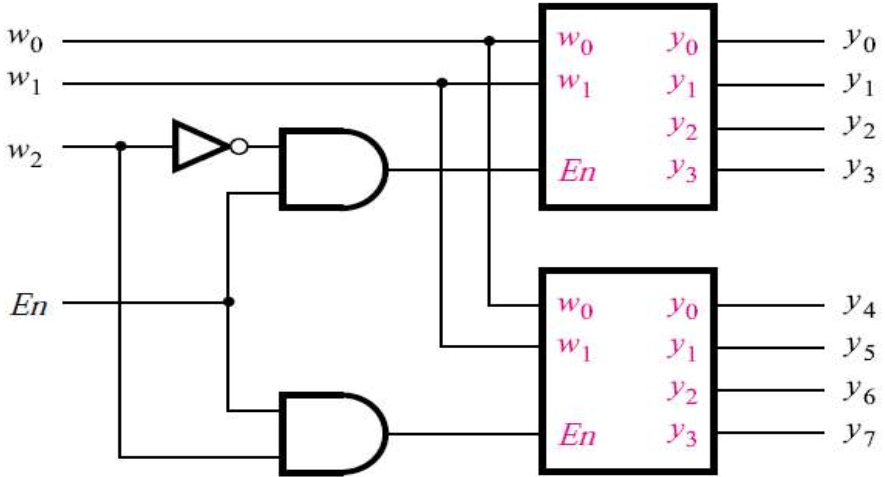
\includegraphics[width=0.5\textwidth]{3 to 8 Decoder using 2 to 4 decoder}
%	\caption{}
	\label{fig:raw data}
\end{figure}


\begin{minted}{vhdl}


Library IEEE;
Use IEEE.std_logic_1164.all;


Entity decoder3to8 is 
   port(w8           :in    std_logic_vector(2 downto 0);
        Enable8      :in    std_logic;
        output8      :out   std_logic_vector(0 to 7));
end decoder3to8;


Architecture Behavior of decoder3to8 is


-- Here we declare an intermediate signal to help us, we use it as intermediate enable

Signal inter_enable :  std_logic_vector(0 to 1);

-- Here we declare a component, our decoder2to4



Component decoder2to4 is 
   port(w           :in    std_logic_vector(1 downto 0);
        Enable      :in    std_logic;
        output      :out   std_logic_vector(0 to 3));
end Component;


begin 

inter_enable(0) <= not w8(2) and Enable8;
inter_enable(1) <= w8(2) and Enable8;

Stage1 : decoder2to4 PORT MAP (w8(1 downto 0), inter_enable(0), output8(0 to 3) );
Stage2 : decoder2to4 PORT MAP (w8(1 downto 0), inter_enable(1), output8(4 to 7) );
end Behavior;

\end{minted}

\item Example: 4 to 1 multiplexer using 2 to 4 decoder:


\begin{figure}[H] 
	\centering
	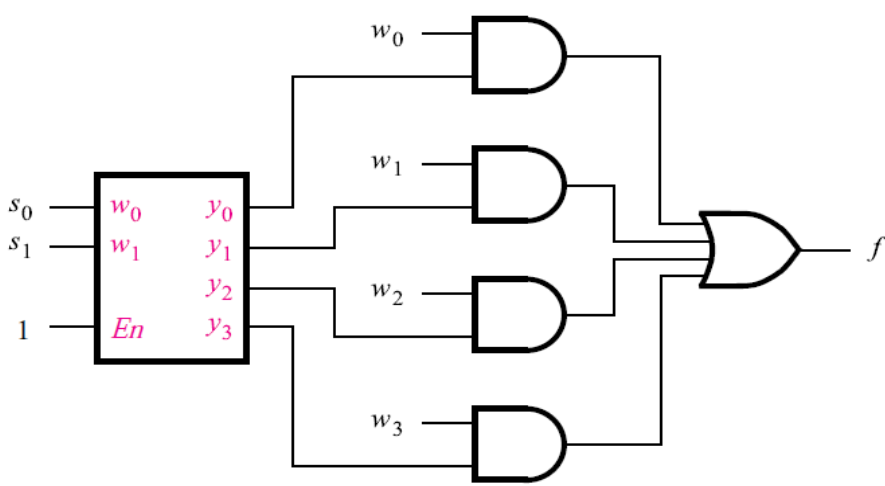
\includegraphics[width=0.5\textwidth]{4 to 1 multiplexer using 2 to 4 decoder}
%	\caption{}
	\label{fig:raw data}
\end{figure}


\begin{minted}{vhdl}


Library IEEE;
Use IEEE.std_logic_1164.all;


Entity mux4to1 is 
   port(w0, w1, w2, w3 :in    std_logic;
        selector       :in    std_logic_vector(1 downto 0);
        output         :out   std_logic);
end mux4to1;


Architecture Behavior of mux4to1 is


-- Here we declare an intermediate signal to help us, we use it to contain the output of the decoder

Signal decoder_output :  std_logic_vector(0 to 3);

-- decoder is always enabled

constant enable : std_logic := '1';

-- Here we declare a component, our decoder2to4



Component decoder2to4 is 
   port(w           :in    std_logic_vector(1 downto 0);
        Enable      :in    std_logic;
        output      :out   std_logic_vector(0 to 3));
end Component;


begin 


Stage : decoder2to4 PORT MAP (selector(1 downto 0), enable, decoder_output(0 to 3) );

with decoder_output select 

   output <= w0 when "1000",
             w1 when "0100",
             w2 when "0010",
             w3 when "0001";

end Behavior;

\end{minted}
\end{itemize}
\end{document}